% Report for Assignment 3: Authorship Attribution (TxMM 2026-2027)
% Limit: 3 pages, self-contained. Submit as Txmm_A3-AA_<groupnumber>.pdf
\documentclass[11pt,twocolumn]{article}
\usepackage[T1]{fontenc}
\usepackage{a4wide}
\usepackage[style=numeric,sorting=none,maxnames=10]{biblatex}
\usepackage[hidelinks]{hyperref}
\usepackage{enumitem}
\usepackage{graphicx}
\usepackage{booktabs}
\usepackage{tabularx}
\usepackage[font=small,skip=4pt]{caption}
\addbibresource{report.bib}
\graphicspath{{../outputs/}}
\setlength{\columnsep}{0.8cm}

\begin{document}

\twocolumn[{
    \vspace*{-1.8cm}
    \begin{center}
        {\Large\bfseries Authorship Attribution}\\[0.3em]
        Text and Multimedia Mining, Assignment 3 \quad--\quad Group 23 \\[0.2em]
        \today
    \end{center}
    \vspace{0.5em}
}]

\section{Introduction and data}
In this paper we train a model to do authorship attribution. Our data is a fragment of the PAN2020 dataset \footnote{\href{https://pan.webis.de/clef20/pan20-web/author-identification.html}{https://pan.webis.de/clef20/pan20-web/author-identification.html}}. The dataset contains fanfiction texts by 20 different authors. To create a model that can automatically predict whether 2 texts were written by the same author, we set up a feature extractor, followed by some classification model. By choosing our features inteligently, and processing them properly, a fairly simple classifier achieves great performance on this task.

\section{Features}

\begin{table}[ht]
    \centering
    \small
    \caption{}
    \label{tab:features}
    \begin{tabularx}{\columnwidth}{@{}lr>{\raggedright\arraybackslash}X@{}}
        \toprule
        Group & \# & Description \\
        \midrule
        Character   & 30 & \\
        Punctuation & 12 & \\
        Structure   &  8 & \\
        Lexical     & 15 & \\
        Syntactic   & 14 & \\
        Informal    & 13 & \\
        Semantic    & 58 & \\
        \midrule
        Total       & 150 & \\
        \bottomrule
    \end{tabularx}
\end{table}

\section{Classifier}
For the classification task, we evaluated several models: a Linear Support Vector Classifier (SVC), a Logistic Regression Model (LRM), and a Random Forest (RF), all implemented using the scikit-learn library. Since many of the input features operate on different scales, and some of these models are sensitive to differences in feature magnitude, we standardized the features using scikit-learn's StandardScaler. This transformation centers each feature around zero and scales it to unit variance. Feature scaling massively improved the F1-score on the development set, as expected.

During early tests, the models had not yet been fully tuned. To improve the performance of the final model, the next step was therefore to optimize the \textit{C} parameter, which controls the degree of regularization applied to the model weights. Since both the SVC and LRM outperformed the RF model, we continued with these two models. In addition to achieving better performance, they are also simpler than the RF model. The results of this tuning process are presented in \ref{fig:c}.

\
\begin{figure}[ht]
    \centering
    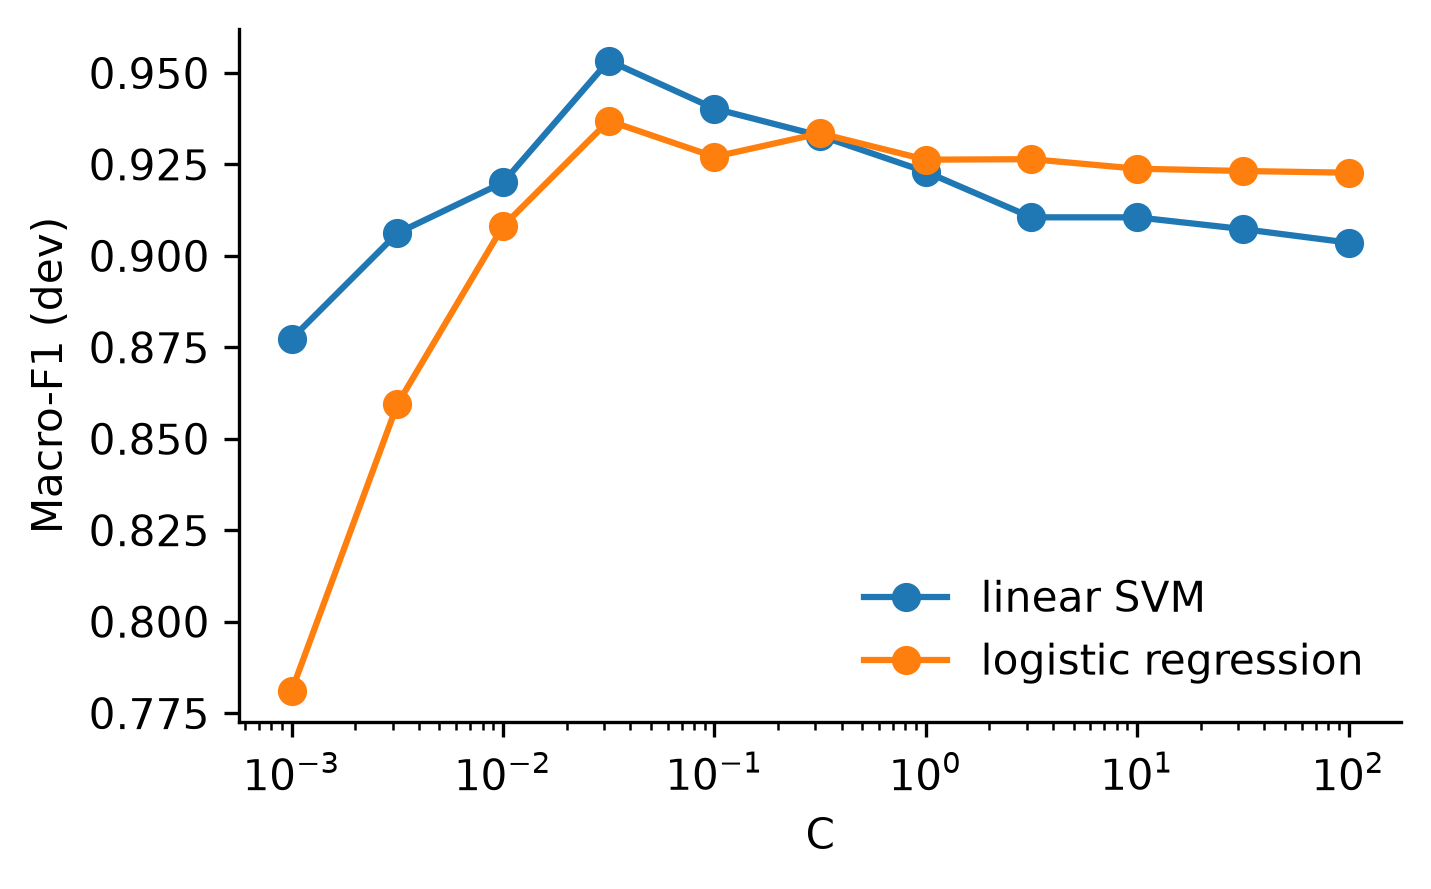
\includegraphics[width=\columnwidth]{tuning_c.png}
    \caption{While the LRM is better with default \textit{c}, the SVC is best with a tuned one.}
    \label{fig:c}
\end{figure}


\section{Results}
Throughout this report, we will evaluate our classifer with the macro-F1 score, the mean F1 over all authors:
\[
    F_1 = \frac{1}{N} \sum_{a=1}^{N} \frac{2 P_a R_a}{P_a + R_a},
\]
where $P_a$ and $R_a$ are the precision and recall for author $a$, and $N = 20$ is the total number of authors.

Standardization is essential for the linear models. Without scaling, the SVC and LRM achieved macro-F1 scores of only 0.731 and 0.386 respectively on the development set. In contrast, the RF model remained unaffected, achieving a macro-F1 score of 0.890. However, after applying the scaler and retaining the default model settings, performance improved substantially: the SVC and LRM reached macro-F1 scores of 0.923 and 0.926 respectively, outperforming the RF model. Tuning C (Figure~\ref{fig:c}) then showed that both linear models perform wbetter with much stronger regularization, as both peak at $C \approx 0.03$ (default $1$). Here, the SVC reaches 0.953. We selected this model, retrained it on the training and development sets combined, and applied it once to the test set.

On the test set, the final model achieves a macro-F1 of 0.944 compared to 0.953 on the development set. This small drop from the development set is expected, since C was selected on it. Furthermore this small of a difference might be covered in noise. Specific mistakes will be discussed in section \ref{sec:discussion}.

\begin{figure}[ht]
    \centering
    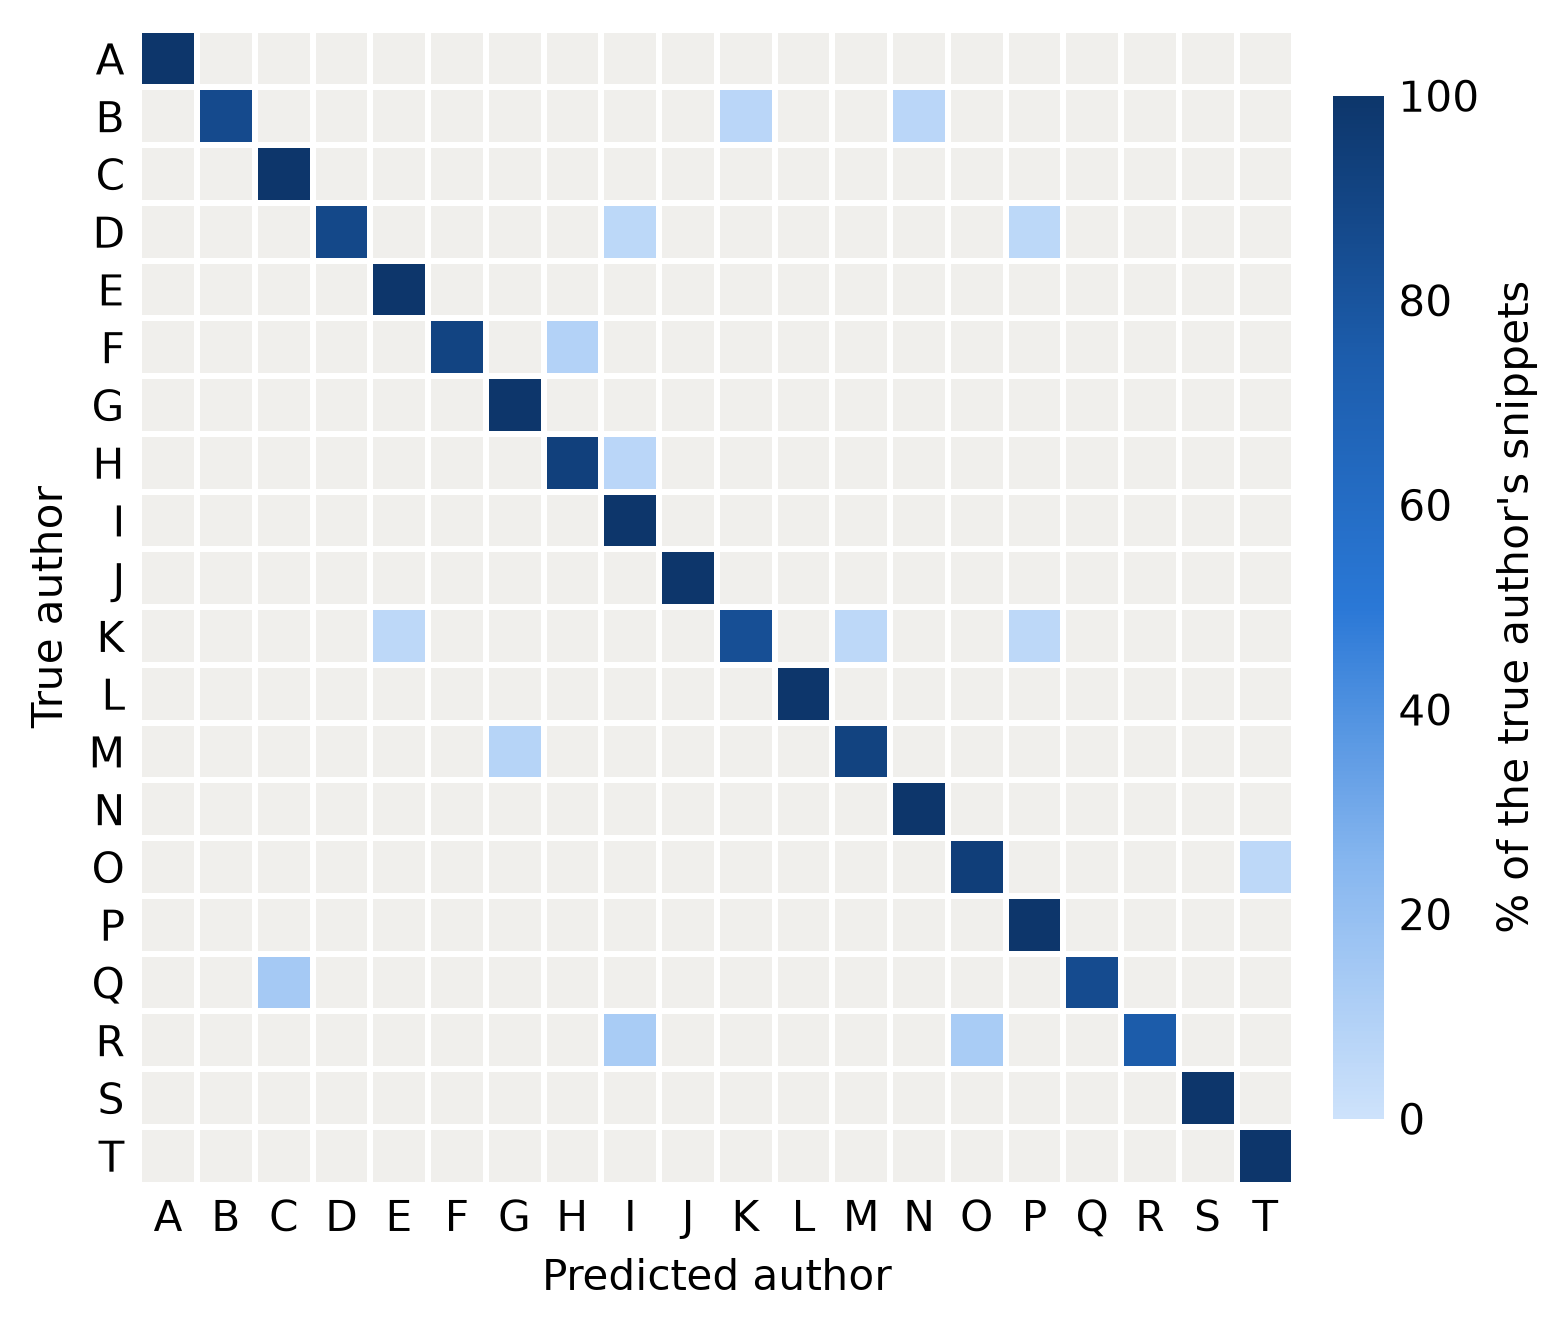
\includegraphics[width=\columnwidth]{confusion_test.png}
    \caption{Confusion matrix of the final SVC on the test set, normalized per true author. Authors are labelled A--T.}
    \label{fig:confusion}
\end{figure}

\section{Ablation and feature selection}
Our final model performed rather well. 

\begin{figure}[ht]
    \centering
    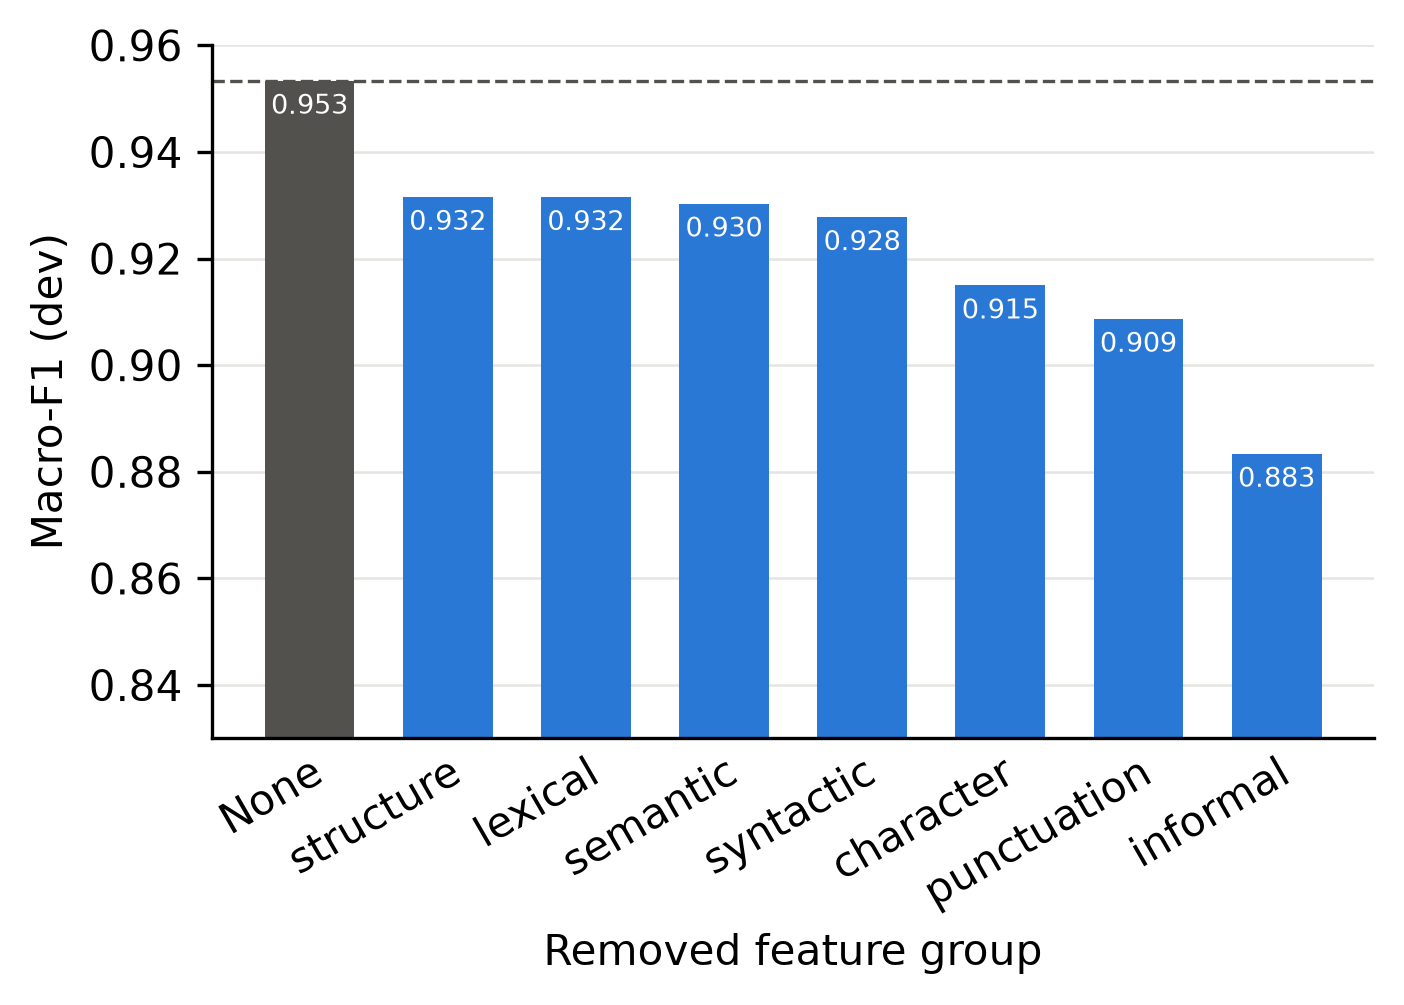
\includegraphics[width=\columnwidth]{ablation.png}
    \caption{Macro-F1 of the final SVC on the development set with one feature group left out. The dark bar uses all features.}
    \label{fig:ablation}
\end{figure}

\section{Discussion}
\label{sec:discussion}

\subsection*{Problems and failure analysis}
% Do failure analysis


\subsection*{With 10 extra hours}

\subsection*{Challenges in authorship attribution}

\section{Conclusion}

\printbibliography

\end{document}
